
%\documentclass[journal]{IEEEtran}


%------------ SCIENCE FORMAT BEGIN -------
\documentclass[12pt]{article}
\usepackage{scicite}
\usepackage{times}

\topmargin 0.0cm
\oddsidemargin 0.2cm
\textwidth 16cm
\textheight 21cm
\footskip 1.0cm

\newenvironment{sciabstract}{%
\begin{quote} \bf}
{\end{quote}}

%------------ SCIENCE FORMAT END -----------
\usepackage{verbatim}
\usepackage{graphicx}
\begin{filecontents*}{biblio.bib}
      @INPROCEEDINGS{4124872,
      author={Alves, J. and Oliveira, P. and Oliveira, R. and Pascoal, A. and Rufino, M. and Sebastiao, L. and Silvestre, C.},
      booktitle={Control and Automation, 2006. MED '06. 14th Mediterranean Conference on},
      title={Vehicle and Mission Control of the DELFIM Autonomous Surface Craft},
      year={2006},
      pages={1-6},
      keywords={data acquisition;marine vehicles;mobile robots;Atlantic;Azores islands;DELFIM autonomous surface craft;ISR/IST;acoustic relay;automatic marine data acquisition;mission control;submerged craft;support vessel;vehicle control;Acoustic testing;Automatic control;Control systems;Data acquisition;Mobile robots;Navigation;Relays;Remotely operated vehicles;Sea surface;Underwater acoustics},
      doi={10.1109/MED.2006.328689},
      month={June},}
      @article{Ettinger2003,
      author = {Ettinger, Sm and Nechyba, Mc and Ifju, Pg and M},
      file = {:home/pulver/Desktop/PhD/Papers/Flying Robots/Towards flight autonomy$\backslash$: vision-based horizon detection for micro air vehicles.pdf:pdf},
      journal = {Florida Conference on},
      number = {17},
      pages = {617--640},
      title = {{Towards flight autonomy: Vision-based horizon detection for micro air vehicles}},
      url = {http://citeseerx.ist.psu.edu/viewdoc/download?doi=10.1.1.16.6951{\&}amp;rep=rep1{\&}amp;type=pdf},
      volume = {7},
      year = {2003}
      }

      @ARTICLE{4082128,
      author={Hart, P.E. and Nilsson, N.J. and Raphael, B.},
      journal={Systems Science and Cybernetics, IEEE Transactions on},
      title={A Formal Basis for the Heuristic Determination of Minimum Cost Paths},
      year={1968},
      volume={4},
      number={2},
      pages={100-107},
      keywords={Automatic control;Automatic programming;Chemical technology;Costs;Functional programming;Gradient methods;Instruction sets;Mathematical programming;Minimax techniques;Minimization methods},
      doi={10.1109/TSSC.1968.300136},
      ISSN={0536-1567},
      month={July},}

      @book{Gonzalez:2001:DIP:559707,
       author = {Gonzalez, Rafael C. and Woods, Richard E.},
       title = {Digital Image Processing},
       year = {2001},
       isbn = {0201180758},
       edition = {2nd},
       publisher = {Addison-Wesley Longman Publishing Co., Inc.},
       address = {Boston, MA, USA},
      }
      @misc{Hough_1962, place={United States}, title={Method and Means for recognizing Complex Patterns}, abstractNote={This patent relates to a method and means for recognizing a complex pattern in a picture.  The picture is divided into framelets, each framelet being sized so that any segment of the complex pattern therewithin is essentially a straight line. Each framelet is scanned to produce an electrical pulse for each point scanned on the segment therewithin. Each of the electrical pulses of each segment is then transformed into a separate strnight line to form a plane transform in a pictorial display. Each line in the plane transform of a segment is positioned laterally so that a point on the line midway between the top and the bottom of the pictorial display occurs at a distance from the left edge of the pictorial display equal to the distance of the generating point in the segment from the left edge of the framelet. Each line in the plane transform of a segment is inclined in the pictorial display at an angle to the vertical whose tangent is proportional to the vertical displacement of the generating point in the segment from the center of the framelet. The coordinate position of the point of intersection of the lines in the pictorial display for each segment is determined and recorded. The sum total of said recorded coordinate positions being representative of the complex pattern. (AEC)}, author={Hough, P.V.C.}, year={1962}, month={Dec}}
      @article{Maini2009,
      abstract = {Automatic image annotation techniques that try to identify the objects in images usually need the images to be segmented first, especially when specifically annotating image regions. The purpose of segmentation is to separate different objects in images from each other, so that objects can be processed as integral individuals. Therefore, annotation performance is highly influenced by the effectiveness of segmentation. Unfortunately, automatic segmentation is a difficult problem, and most of the current segmentation techniques do not guarantee good results. A multiple segmentations algorithm is proposed by Russell et al. [12] to discover objects and their extent in images. In this paper, we explore the novel use of multiple segmentations in the context of image auto-annotation. It is incorporated into a region based image annotation technique proposed in previous work, namely the training image based feature space approach. Three different levels of segmentations were generated for a 5000 image collection. Experimental results show that image auto-annotation achieves better performance when using all three segmentation levels together than using any single one on its own.},
      author = {Maini, Raman and Aggarwal, H},
      file = {:home/pulver/Dropbox/Universit{\`{a}}/PhD/Image processing/Study and comparison of various imahe edge detection techniques.pdf:pdf},
      journal = {International Journal of Image Processing {\ldots}},
      keywords = {digital image processing,edge detection,noise},
      number = {3},
      pages = {1--12},
      title = {{Study and comparison of various image edge detection techniques}},
      url = {http://wwwmath.tau.ac.il/{~}turkel/notes/Maini.pdf},
      volume = {147002},
      year = {2009}
      }

      @article{Fischler1981,
      abstract = {A new paradigm, Random Sample Consensus (RANSAC), for fitting a model to experimental data is introduced. RANSAC is capable of interpreting/ smoothing data containing a significant percentage of gross errors, and is thus ideally suited for applications in automated image analysis where interpretation is based on the data provided by error-prone feature detectors. A major portion of this paper describes the application of RANSAC to the Location Determination Problem (LDP): Given an image depicting a set of landmarks with known locations, determine that point in space from which the image was obtained. In response to a RANSAC requirement, new results are derived on the minimum number of landmarks needed to obtain a solution, and algorithms are presented for computing these minimum-landmark solutions in closed form. These results provide the basis for an automatic system that can solve the LDP under difficult viewing and analysis conditions. Implementation details and computational examples are also presented.},
      author = {Fischler, Martin a and Bolles, Robert C},
      doi = {10.1145/358669.358692},
      file = {:home/pulver/Desktop/PhD/Papers/Obstacle detection/ransac.pdf:pdf},
      isbn = {0934613338},
      issn = {0001-0782},
      journal = {Communications of the ACM},
      keywords = {automated cartography,camera calibration,computer{\_}vision,epipolar,geometry,image matching,keypoints,location determination,match-rejection,model fitting,motion-estimation,multi-view,rpc,scene analysis,sift,stereo,structure{\_}from{\_}motion,tracking},
      number = {6},
      pages = {381 -- 395},
      title = {{Random Sample Consensus: A Paradigm for Model Fitting with Applicatlons to Image Analysis and Automated Cartography}},
      volume = {24},
      year = {1981}
      }

      @article{EWD:NumerMath59,
      author = {Edsger. W. Dijkstra},
      title = {A note on two problems in connexion with graphs.},
      year = {1959},
      journal = {Numerische Mathematik},
      volume = {1},
      pages = {269--271},
      }


      @article{Naeem2009,
      abstract = {An adaptive navigation and control algorithm is presented in this paper based on fuzzy logic and optimal control techniques and applied on an unmanned surface vehicle platform. The navigation system consists of an extended Kalman filter with time-varying parameters. Whilst the autopilots include a fuzzy logic based linear quadratic Gaussian controller and a model predictive controller optimized using a genetic algorithm. Both the controllers use the output of the adaptive navigation system as their feedback and therefore creates an integrated system. A multiple waypoint following scenario is considered and tested in real time. Experimental results are shown that demonstrate the efficacy of the proposed system.},
      author = {Naeem, W. and Sutton, R.},
      doi = {10.1049/cp.2009.1686},
      file = {:home/pulver/.local/share/data/Mendeley Ltd./Mendeley Desktop/Downloaded/Naeem, Sutton - 2009 - An intelligent integrated navigation and control solution for an unmanned surface craft.pdf:pdf},
      isbn = {978 1 84919 213 2},
      journal = {IET Irish Signals and Systems Conference (ISSC 2009)},
      keywords = {Kalman filter,LQG,covariance matrices,guidance,model predictive control,unmanned surface vehicles},
      pages = {9--9},
      title = {{An intelligent integrated navigation and control solution for an unmanned surface craft}},
      url = {http://ieeexplore.ieee.org/xpls/abs{\_}all.jsp?arnumber=5524711' escapeXml='false'/>},
      year = {2009}
      }
      @article{Bertram2008,
      abstract = {The survey of marine Unmanned Surface Vehicles (USVs) covers both actually built and projected USVs. Most USV developments are found in the USA. USVs remain so far limited to small to medium vessels with limited autonomy.},
      author = {Bertram, Volker},
      file = {:home/pulver/.local/share/data/Mendeley Ltd./Mendeley Desktop/Downloaded/Bertram - 2008 - Unmanned Surface Vehicles – A Survey.pdf:pdf},
      journal = {Skibsteknisk Selskab, Copenhagen, Denmark},
      pages = {1--14},
      title = {{Unmanned Surface Vehicles : A Survey}},
      year = {2008}
      }
      @article{Khatib1985,
      author = {Khatib, O.},
      doi = {10.1109/ROBOT.1985.1087247},
      file = {:home/pulver/Dropbox/Universit{\`{a}}/PhD/Path Planning/Real-time Obstacle Avoidance for manipulatos and mobile robots.pdf:pdf},
      journal = {Proceedings. 1985 IEEE International Conference on Robotics and Automation},
      pages = {500--505},
      title = {{Real-time obstacle avoidance for manipulators and mobile robots}},
      volume = {2},
      year = {1985}
      }

      @inproceedings{Tan2010,
      abstract = {In this paper, an obstacle avoidance solution based on rules and criteria is presented. The solution has two parts. In the first part, a set of candidate maneuvers is generated to track a given path. Each candidate differs in speed and in lateral offset to the tracked path. Thus, the USV has the option to change speeds or switch "lanes", or do both. In the second part, the most appropriate trajectory is selected for execution. High priority objectives, such as safety clearance, are represented quantitatively as rules. Candidate maneuvers that flout any of these rules are immediately rejected. Lower priority objectives, such as minimizing travel time, are represented as a priority list of selection criteria. From the remaining candidates, an iterative process of short listing maneuvers is performed. At each step, a single criterion is used to rank and select the top trajectories. The process is repeated for criteria of decreasing priority until only one maneuvers remains. The presented solution has been implemented and tested in simulation. Some of these simulation results will be presented.},
      author = {Tan, Aaron and Wee, Wong Chee and Tan, Timothy Joe},
      booktitle = {2010 International WaterSide Security Conference},
      doi = {10.1109/WSSC.2010.5730288},
      file = {:home/pulver/Dropbox/Universit{\`{a}}/PhD/Marine Robotic Overview/Obstacle avoidance/Criteria and rule based obstacle avoidaance for usv.pdf:pdf},
      isbn = {978-1-4244-8894-0},
      pages = {1--6},
      title = {{Criteria and rule based obstacle avoidance for USVs}},
      year = {2010}
      }

      @article{Sorbara2015,
      author = {Sorbara, Andrea and Odetti, Angelo and Bibuli, Marco and Zereik, Enrica and Bruzzone, Gabriele},
      file = {:home/pulver/Dropbox/Universit{\`{a}}/PhD/Marine Robotic Overview/Obstacle avoidance/Design of an obstacle detection system for marine autonomous vehicles.pdf:pdf},
      isbn = {9781479987368},
      keywords = {marine vehicles,obstacle detection,optronic},
      title = {{Design of an Obstacle Detection System for Marine Autonomous Vehicles}},
      year = {2015}
      }
      @article{Schuster2014,
      author = {Schuster, Michael and Blaich, Michael and Reuter, Johannes},
      file = {:home/pulver/Dropbox/Universit{\`{a}}/PhD/Marine Robotic Overview/Obstacle avoidance/Collision Avoidance for Vessels using a Low-Cost Radar Sensor.pdf:pdf},
      keywords = {collision avoidance,colregs,interacting multiple model filter,path planning,raster grid,ship navigation},
      number = {2009},
      pages = {9673--9678},
      title = {{Collision Avoidance for Vessels using a Low-Cost Radar Sensor}},
      year = {2014}
      }
      @inproceedings{Achanta2009,
      abstract = {Detection of visually salient image regions is useful for applications like object segmentation, adaptive compression, and object recognition. In this paper, we introduce a method for salient region detection that outputs full resolution saliency maps with well-defined boundaries of salient objects. These boundaries are preserved by retaining substantially more frequency content from the original image than other existing techniques. Our method exploits features of color and luminance, is simple to implement, and is computationally efficient. We compare our algorithm to five state-of-the-art salient region detection methods with a frequency domain analysis, ground truth, and a salient object segmentation application. Our method outperforms the five algorithms both on the ground-truth evaluation and on the segmentation task by achieving both higher precision and better recall.},
      author = {Achanta, Radhakrishna and Hemami, Sheila and Estrada, Francisco and Susstrunk, S},
      booktitle = {Computer Vision and Pattern Recognition, 2009. CVPR 2009. IEEE Conference on},
      doi = {10.1109/CVPR.2009.5206596},
      file = {:home/pulver/Dropbox/Universit{\`{a}}/PhD/Obstacle detection/Frequency-tuned Salient Region Detection.pdf:pdf},
      isbn = {1063-6919 VO -},
      issn = {1063-6919},
      keywords = {Biological system modeling,Biology computing,Frequency domain analysis,Frequency estimation,Image analysis,Image coding,Image segmentation,Object detection,Object recognition,Object segmentation,color,edge detection,frequency-tuned salient region detection,full resolution saliency map,image colour analysis,image resolution,luminance,visual saliency},
      number = {Ic},
      pages = {1597--1604},
      pmid = {5206596},
      title = {{Frequency-tuned salient region detection}},
      year = {2009}
      }

      @article{Harris1988,
      abstract = {Consistency of image edge filtering is of prime importance for 3D interpretation of image sequences using feature tracking algorithms. To cater for image regions containing texture and isolated features, a combined corner and edge detector based on the local auto-correlation function is utilised, and it is shown to perform with good consistency on natural imagery.},
      author = {Harris, C. and Stephens, M.},
      doi = {10.5244/C.2.23},
      file = {:home/pulver/Dropbox/Universit{\`{a}}/PhD/Obstacle detection/A combined corner and edge detector.pdf:pdf},
      issn = {09639292},
      journal = {Procedings of the Alvey Vision Conference 1988},
      pages = {147--151},
      pmid = {20130988},
      title = {{A Combined Corner and Edge Detector}},
      year = {1988}
      }
      @article{Bouguet1999,
      abstract = {Pyramid LK $\Upsilon$르},
      archivePrefix = {arXiv},
      arxivId = {3629719},
      author = {Bouguet, Jean-yves},
      doi = {10.1016/j.tim.2005.08.009},
      eprint = {3629719},
      file = {:home/pulver/Dropbox/Universit{\`{a}}/PhD/Obstacle detection/Pyramidal Implementation of the Lucas Kanade feature tracker.pdf:pdf},
      isbn = {0966-842X (Print)$\backslash$n0966-842X (Linking)},
      issn = {0966842X},
      journal = {In Practice},
      number = {2},
      pages = {1--9},
      pmid = {16140533},
      title = {{Pyramidal Implementation of the Lucas Kanade Feature Tracker Description of the algorithm}},
      volume = {1},
      year = {1999}
      }


      @article{Almeida2009,
      abstract = {Abstract- This work presents the integration of obstacle detection and analysis capabilities in a coherent and advanced C{\&}C framework allowing mixed-mode control in unmanned surface systems. The collision avoidance work has been successfully integrated in an operational autonomous surface vehicle and demonstrated in real operational conditions. We present the collision avoidance system, the ROAZ autonomous surface vehicle and the results obtained at sea tests. Limitations of current COTS radar systems are also discussed and further research directions are proposed towards the development and integration of advanced collision avoidance systems taking in account the different requirements in unmanned surface vehicles},
      author = {Almeida, Carlos and Franco, Tiago and Ferreira, Hugo and Martins, Alfredo and Santos, Ricardo and Almeida, Jos{\'{e}} Miguel and Silva, Eduardo},
      doi = {10.1109/OCEANSE.2009.5278238},
      file = {:home/pulver/.local/share/data/Mendeley Ltd./Mendeley Desktop/Downloaded/Almeida et al. - 2009 - Radar Based Collision detection developments on USV ROAZ II.pdf:pdf},
      isbn = {978-1-4244-2522-8},
      journal = {Oceans09 Bremen},
      pages = {1--6},
      title = {{Radar Based Collision detection developments on USV ROAZ II}},
      year = {2009}
      }
      @article{Wang2011,
      abstract = {This paper describes a vision-based obstacle detection system for Unmanned Surface Vehicle (USV) towards the aim of real-time and high performance obstacle detection on the sea surface. By using both the monocular and stereo vision methods, the system offers the capacity of detecting and locating multiple obstacles in the range from 30 to 100 meters for high speed USV which runs at speeds up to 12 knots. Field tests in the real scenes have been taken and the obstacle detection system for USV is proven to provide stable and satisfactory performance.},
      author = {Wang, Han and Wei, Zhuo and Wang, Sisong and Ow, Chek Seng and Ho, Kah Tong and Feng, Benjamin},
      doi = {10.1109/RAMECH.2011.6070512},
      file = {:home/pulver/Dropbox/Universit{\`{a}}/PhD/Marine Robotic Overview/Obstacle avoidance/A vision based obstacle detection system for unmanned surface Vehicle.pdf:pdf},
      isbn = {9781612842509},
      issn = {2158219X},
      journal = {IEEE Conference on Robotics, Automation and Mechatronics, RAM - Proceedings},
      keywords = {Unmanned Surface Vehicle (USV),computer vision,obstacle detection},
      pages = {364--369},
      title = {{A vision-based obstacle detection system for unmanned surface vehicle}},
      year = {2011}
      }
      @article{Azzabi,
      author = {Azzabi, Tarek},
      doi = {10.1109/CISTEM.2014.7076748},
      file = {:home/pulver/Dropbox/Universit{\`{a}}/PhD/Marine Robotic Overview/Obstacle avoidance/Obstacle detection for unmanned surface vehicle.pdf:pdf},
      isbn = {9781479973002},
      keywords = {calculate the distance,experimentation results,flow,horizon line detection,matlab simulink,obstacle detection,optical,part will summarize the,the approaches used to,usv,while the forth},
      number = {5},
      pages = {1--7},
      title = {{Obstacle detection for Unmanned Surface Vehicle}},
      year = {2014}
      }
      @article{Wang2012,
      author = {Wang, Han and Wei, Zhuo},
      file = {:home/pulver/Dropbox/Universit{\`{a}}/PhD/Marine Robotic Overview/Obstacle avoidance/Improvement in real time obstacle detection system for usv.pdf:pdf},
      isbn = {9781467318723},
      keywords = {benjamin feng,chek seng ow,computer vision,junjie,kah tong ho,obstacle detection,surface vehicle,unmanned,usv},
      number = {December},
      pages = {5--7},
      title = {{Improvement in Real-time Obstacle Detection System for USV}},
      volume = {2012},
      year = {2012}
      }
      @article{Feng2011,
      abstract = {This paper presents a real-time obstacle detection system for obstacle detection on the sea surface for Unmanned Surface Vehicle (USV). The system employs both monocular and stereo vision-based methods and offers the capacity of detecting and locating multiple obstacles in the range from 30 to 100 meters for high speed USV. Field tests have been taken and shown that the real-time obstacle detection system for USV can provide stable and satisfactory performance.},
      author = {Feng, Benjamin},
      doi = {10.1109/DSR.2011.6026880},
      file = {:home/pulver/Dropbox/Universit{\`{a}}/PhD/Marine Robotic Overview/Obstacle avoidance/Real time obstacle detection for unmanned surface vehicle.pdf:pdf},
      isbn = {978-1-4244-9276-3},
      journal = {2011 Defense Science Research Conference and Expo (DSR)},
      keywords = {1,achieve real-time processing,computer vision,created a graphical user,fig,for ease of use,interface for the system,obstacle detection,surface vehicle,unmanned,usv,we have},
      pages = {1--4},
      title = {{Real-time obstacle detection for Unmanned Surface Vehicle}},
      year = {2011}
      }

      @article{Azzabi,
      author = {Azzabi, Tarek},
      doi = {10.1109/CISTEM.2014.7076748},
      file = {:home/pulver/Dropbox/Universit{\`{a}}/PhD/Marine Robotic Overview/Obstacle avoidance/Obstacle detection for unmanned surface vehicle.pdf:pdf},
      isbn = {9781479973002},
      keywords = {calculate the distance,experimentation results,flow,horizon line detection,matlab simulink,obstacle detection,optical,part will summarize the,the approaches used to,usv,while the forth},
      number = {5},
      pages = {1--7},
      title = {{Obstacle detection for Unmanned Surface Vehicle}}
      }
      @article{Blaich2015,
      author = {Blaich, Michael and Koehler, Steffen and Schuster, Michael and Reuter, Johannes and Tietz, Thomas},
      file = {:home/pulver/Dropbox/Universit{\`{a}}/PhD/Marine Robotic Overview/Obstacle avoidance/Mission integrated collision avoidance for usv using laser range finder.pdf:pdf},
      isbn = {9781479987368},
      journal = {Oceans 2015 Mts/Ieee},
      pages = {0--5},
      title = {{Mission Integrated Collision Avoidance for USVs using Laser Ranger}},
      year = {2015}
      }
      @article{Casalino2009,
      abstract = {The use of unmanned vehicles in the field of underwater and marine applications is increasing significantly in recent years. Autonomous vehicles (like AUVs and gliders) or teleoperated ones (like ROVs) are currently employed for executing a number of different underwater tasks, like inspecting submerged pipes, executing maintenance interventions on underwater gas- or oil-platforms, collecting environmental or oceanographic data, performing surveys on sites of archeological interest. In parallel with the development of underwater vehicles, unmanned surface vehicles (USVs), are they also witnessing an increasing interest from the robotic community, especially with the goal of performing surveillance applications, like patrolling and maintaining safeguarded against intruders harbours or other ldquocrucialrdquo sites. The potential benefits offered by automated vessels equipped with sensors such as cameras or sonars are quite evident, since they could be used to quickly identify the level of menace of unknown radar track without exposing any human operators to possible threats. However USVs, unlike in the underwater case, have to face the problem of avoiding other vessels which in most cases are manned ones. This is a crucial point especially in that kind of application, where the automated vessel has to move quickly towards a possible menace while at the same time avoiding all the other boats normally operating in the harbour area. Unfortunately, at the current state of art, a reliable methodology to avoid the other vessels and the availability of effective and accurate obstacle detection sensors is still missing. This paper focus its attention on the case of USV used for security applications within a harbour, devising a solution that can be real-time implemented for the obstacle avoidance problem under critical situations where the vehicle as to reach its target as fast as possible while guaranteeing the safety of the other vessels. The presented solution is based on- a three layered hierarchical architecture: the first layer computes a global path taking into account static obstacles known a priori, the second layer modifies this path in a locally optimal way (under certain assumptions) exploiting kinematic data of the moving obstacles, while the last layer reactively avoids obstacles for which such data is not available. The paper was therefore organized as follows: in the first section an introduction and state of art are presented, in the successive section the work discussed the first layer and the methods for the static obstacles avoidance, while in the third the paper focused on the moving obstacles and the proposed avoidance algorithm, while also presenting many different detailed simulation results regarding the performances achievable by the overall architecture. Finally a concluding section also indicate some still open problems and future work directions to be developed.},
      author = {Casalino, Giuseppe and Turetta, Alessio and Simetti, Enrico},
      doi = {10.1109/OCEANSE.2009.5278104},
      file = {:home/pulver/Dropbox/Universit{\`{a}}/PhD/Marine Robotic Overview/Obstacle avoidance/A three layered architecture for real time path planning and obstacle avoidance for surveillance usv operating in harbour fields.pdf:pdf},
      isbn = {978-1-4244-2522-8},
      journal = {Oceans 2009-Europe},
      keywords = {AUVs,Art,Marine vehicles,Mobile robots,Path planning,ROV,Radar tracking,Remotely operated vehicles,Sea surface,Surveillance,Underwater vehicles,Vehicle safety,autonomous vehicles,collision avoidance,gliders,harbour fields,kinematic data,marine application,marine safety,mobile robots,obstacle avoidance problem,obstacle detection sensors,radar,real time path planning,remotely operated vehicles,robot kinematics,robotic,security,security applications,surveillance,surveillance unmanned surface vehicles,teleoperated vehicles,telerobotics,three-layered architecture,underwater application,underwater vehicles},
      pages = {1--8},
      title = {{A three-layered architecture for real time path planning and obstacle avoidance for surveillance USVs operating in harbour fields}},
      year = {2009}
      }
      @article{Kuwata2014,
      abstract = {This paper presents an autonomous motion planning algorithm for unmanned surface vehicles (USVs) to navigate safely in dynamic, cluttered environments. The algorithm not only addresses hazard avoidance (HA) for stationary and moving hazards, but also applies the International Regulations for Preventing Collisions at Sea (known as COLREGS, for COLlision REGulationS). The COLREGS rules specify, for example, which vessel is responsible for giving way to the other and to which side of the 'stand-on' vessel to maneuver. Three primary COLREGS rules are considered in this paper: crossing, overtaking, and head-on situations. For autonomous USVs to be safely deployed in environments with other traffic boats, it is imperative that the USV's navigation algorithm obeys COLREGS. Furthermore, when other boats disregard their responsibility under COLREGS, the USV must fall back to its HA algorithms to prevent a collision. The proposed approach is based on velocity obstacles (VO) method, which generates a cone-shaped obstacle in the velocity space. Because VOs also specify on which side of the obstacle the vehicle will pass during the avoidance maneuver, COLREGS are encoded in the velocity space in a natural way. Results from several experiments involving up to four vessels are presented, in what we believe is the first on-water demonstration of autonomous COLREGS maneuvers without explicit intervehicle communication. We also show an application of this motion planner to a target trailing task, where a strategic planner commands USV waypoints based on high-level objectives, and the local motion planner ensures hazard avoidance and compliance with COLREGS during a traverse. © 2013 IEEE.},
      author = {Kuwata, Yoshiaki and Wolf, Michael T. and Zarzhitsky, Dimitri and Huntsberger, Terrance L.},
      doi = {10.1109/JOE.2013.2254214},
      file = {:home/pulver/.local/share/data/Mendeley Ltd./Mendeley Desktop/Downloaded/Kuwata et al. - 2014 - Safe Maritime Autonomous Navigation With COLREGS, Using Velocity Obstacles.pdf:pdf},
      isbn = {978-1-61284-455-8},
      issn = {0364-9059},
      journal = {IEEE Journal of Oceanic Engineering},
      keywords = {COLREGS,unmanned surface vehicle (USV),velocity obstacles (VOs)},
      number = {1},
      pages = {110--119},
      title = {{Safe Maritime Autonomous Navigation With COLREGS, Using Velocity Obstacles}},
      volume = {39},
      year = {2014}
      }
      @article{Kuwata2014a,
      abstract = {This paper presents an autonomous motion planning algorithm for unmanned surface vehicles (USVs) to navigate safely in dynamic, cluttered environments. The algorithm not only addresses hazard avoidance (HA) for stationary and moving hazards, but also applies the International Regulations for Preventing Collisions at Sea (known as COLREGS, for COLlision REGulationS). The COLREGS rules specify, for example, which vessel is responsible for giving way to the other and to which side of the 'stand-on' vessel to maneuver. Three primary COLREGS rules are considered in this paper: crossing, overtaking, and head-on situations. For autonomous USVs to be safely deployed in environments with other traffic boats, it is imperative that the USV's navigation algorithm obeys COLREGS. Furthermore, when other boats disregard their responsibility under COLREGS, the USV must fall back to its HA algorithms to prevent a collision. The proposed approach is based on velocity obstacles (VO) method, which generates a cone-shaped obstacle in the velocity space. Because VOs also specify on which side of the obstacle the vehicle will pass during the avoidance maneuver, COLREGS are encoded in the velocity space in a natural way. Results from several experiments involving up to four vessels are presented, in what we believe is the first on-water demonstration of autonomous COLREGS maneuvers without explicit intervehicle communication. We also show an application of this motion planner to a target trailing task, where a strategic planner commands USV waypoints based on high-level objectives, and the local motion planner ensures hazard avoidance and compliance with COLREGS during a traverse. © 2013 IEEE.},
      author = {Kuwata, Yoshiaki and Wolf, Michael T. and Zarzhitsky, Dimitri and Huntsberger, Terrance L.},
      doi = {10.1109/JOE.2013.2254214},
      file = {:home/pulver/Dropbox/Universit{\`{a}}/PhD/Marine Robotic Overview/Obstacle avoidance/Safe maritime navigation with COLREGS using velocity obstacles.pdf:pdf},
      isbn = {978-1-61284-455-8},
      issn = {0364-9059},
      journal = {IEEE Journal of Oceanic Engineering},
      keywords = {COLREGS,unmanned surface vehicle (USV),velocity obstacles (VOs)},
      number = {1},
      pages = {110--119},
      title = {{Safe Maritime Autonomous Navigation With COLREGS, Using Velocity Obstacles}},
      volume = {39},
      year = {2014}
      }
      @article{Larson2007,
      author = {Larson, Jacoby and Bruch, Michael and Ebken, John and Warfare, Naval and Diego, San and Diego, San},
      file = {:home/pulver/Dropbox/Universit{\`{a}}/PhD/Marine Robotic Overview/Autonomous navigation and obstacle avoidance for unmanned surface vehicles.pdf:pdf},
      isbn = {6195539775},
      keywords = {autonomous,obstacle avoidance,path,robotics,unmanned surface vehicle,usv,waypoint navigation},
      pages = {17--20},
      title = {{Autonomous Navigation and Obstacle avoidance for unmanned surface vehicles}},
      year = {2007}
      }
      @article{Larson2007a,
      abstract = {The Space and Naval Warfare Systems Center, San Diego has been involved in the continuing development of obstacle avoidance for unmanned surface vehicles (USVs) towards the aim of a high level of autonomous navigation. An autonomous USV can fulfill a variety of missions and applications that are of increasing interest for the US Navy and other Department of Defense and Department of Homeland Security organizations. The USV obstacle avoidance package is being developed first by accurately creating a world model based on various sensors such as vision, radar, and nautical charts. Then, with this world model the USV can avoid obstacles with the use of a far-field deliberative obstacle avoidance component and a near-field reactive obstacle avoidance component. This paper addresses the advances made in USV obstacle avoidance during the last two years.},
      author = {Larson, Jacoby and Bruch, Michael and Halterman, Ryan and Rogers, John and Webster, Robert},
      file = {:home/pulver/.local/share/data/Mendeley Ltd./Mendeley Desktop/Downloaded/Larson et al. - 2007 - Advances in Autonomous Obstacle Avoidance for Unmanned Surface Vehicles.pdf:pdf},
      isbn = {6195539775},
      journal = {Techniques},
      keywords = {autonomous,oa,obstacle avoidance,path planning,reactive,robotics,unmanned surface vehicle,usv},
      pages = {1--15},
      title = {{Advances in Autonomous Obstacle Avoidance for Unmanned Surface Vehicles}},
      year = {2007}
      }
      @article{Leng2013,
      abstract = {This paper presents an algorithm for online path planning of USVs to navigate safely in dynamic, sophisticated environments of oceans. The proposed algorithm is based on Mixed Integer Linear Programming (MILP) which integrated with Velocity Obstacle (VO) approach. MILP is an optimization method under multiple constraint conditions of objective function maximization or minimization. The constraints of environment and maneuverability all can be considered and appended to the constraints conditions expressed in the form of inequality. The objective function and constraint conditions are required in linear by MILP, however, the motion of USV and its path planning are nonlinear. So the principle problem is to transform the nonlinear problem into the linear problem. On the other hand, VO makes a linear prediction, which is well appended into the constraint conditions. MILP has advantages in astringency, optimization, real-time and VO also has the advantages in real-time. The combination of MILP and VO utilized the advantages of rapidity of computations, which is well suited for embedded system of robotic applications. The algorithm is demonstrated via simulation with more safety and acclimation in sophisticated environments of oceans.},
      author = {Leng, Jing and Liu, Jian and Xu, Hongli},
      file = {:home/pulver/.local/share/data/Mendeley Ltd./Mendeley Desktop/Downloaded/Leng, Liu, Xu - 2013 - Online path planning based on MILP for unmanned surface vehicles.pdf:pdf},
      isbn = {VO  -},
      journal = {Oceans - San Diego, 2013},
      keywords = {Collision avoidance,Heuristic algorithms,Linear programming,MILP,Mathematical model,Online path planning,Optimization,Trajectory,USV,Velocity Obstacle,integer programming,linear programming,marine vehicles,minimisation,mixed integer linear programming,nonlinear problem,objective function maximization,objective function minimization,oceans,online path planning,optimization method,path planning,remotely operated vehicles,unmanned surface vehicle,velocity obstacle},
      pages = {1--7},
      title = {{Online path planning based on MILP for unmanned surface vehicles}},
      year = {2013}
      }
      @article{Schuster2014,
      author = {Schuster, Michael and Blaich, Michael and Reuter, Johannes},
      file = {:home/pulver/Dropbox/Universit{\`{a}}/PhD/Marine Robotic Overview/Obstacle avoidance/Collision Avoidance for Vessels using a Low-Cost Radar Sensor.pdf:pdf},
      keywords = {collision avoidance,colregs,interacting multiple model filter,path planning,raster grid,ship navigation},
      number = {2009},
      pages = {9673--9678},
      title = {{Collision Avoidance for Vessels using a Low-Cost Radar Sensor}},
      year = {2014}
      }
      @article{Simetti2014,
      author = {Simetti, Enrico and Torelli, Sandro and Casalino, Giuseppe and Turetta, Alessio},
      file = {:home/pulver/Dropbox/Universit{\`{a}}/PhD/Marine Robotic Overview/Obstacle avoidance/Experimental results on obstacle avoidance for high speed unmanned surface vehicles.pdf:pdf},
      isbn = {9781479949182},
      pages = {0--5},
      title = {{Experimental Results on Obstacle Avoidance for High Speed Unmanned Surface Vehicles}},
      year = {2014}
      }
      @article{Sorbara2015,
      author = {Sorbara, Andrea and Odetti, Angelo and Bibuli, Marco and Zereik, Enrica and Bruzzone, Gabriele},
      file = {:home/pulver/Dropbox/Universit{\`{a}}/PhD/Marine Robotic Overview/Obstacle avoidance/Design of an obstacle detection system for marine autonomous vehicles.pdf:pdf},
      isbn = {9781479987368},
      keywords = {marine vehicles,obstacle detection,optronic},
      title = {{Design of an Obstacle Detection System for Marine Autonomous Vehicles}},
      year = {2015}
      }
      @article{Tang2012,
      author = {Tang, Pingpeng and Zhang, Rubo and Liu, Deli and Zou, Qijie and Shi, Changting},
      doi = {10.1109/CCDC.2012.6244200},
      file = {:home/pulver/Dropbox/Universit{\`{a}}/PhD/Marine Robotic Overview/Obstacle avoidance/Research od Neaf field obstacle avoidance for unmanned surface vehicle based on heading window.pdf:pdf},
      isbn = {9781457720727},
      journal = {Proceedings of the 2012 24th Chinese Control and Decision Conference, CCDC 2012},
      keywords = {"Divide and Conquer" Strategy,Dynamic Window method,Heading Window,Near-Field Obstacle-Avoidance,Tangent-Method,USV(Unmanned Surface Vehicle)},
      pages = {1262--1267},
      title = {{Research on near-field obstacle avoidance for unmanned surface vehicle based on heading window}},
      year = {2012}
      }
      @article{Wang2011,
      abstract = {This paper describes a vision-based obstacle detection system for Unmanned Surface Vehicle (USV) towards the aim of real-time and high performance obstacle detection on the sea surface. By using both the monocular and stereo vision methods, the system offers the capacity of detecting and locating multiple obstacles in the range from 30 to 100 meters for high speed USV which runs at speeds up to 12 knots. Field tests in the real scenes have been taken and the obstacle detection system for USV is proven to provide stable and satisfactory performance.},
      author = {Wang, Han and Wei, Zhuo and Wang, Sisong and Ow, Chek Seng and Ho, Kah Tong and Feng, Benjamin},
      doi = {10.1109/RAMECH.2011.6070512},
      file = {:home/pulver/Dropbox/Universit{\`{a}}/PhD/Marine Robotic Overview/Obstacle avoidance/A vision based obstacle detection system for unmanned surface Vehicle.pdf:pdf},
      isbn = {9781612842509},
      issn = {2158219X},
      journal = {IEEE Conference on Robotics, Automation and Mechatronics, RAM - Proceedings},
      keywords = {Unmanned Surface Vehicle (USV),computer vision,obstacle detection},
      pages = {364--369},
      title = {{A vision-based obstacle detection system for unmanned surface vehicle}},
      year = {2011}
      }
      @article{Xie2014,
      author = {Xie, Shaorong and Wu, Peng and Peng, Yan and Luo, Jun and Gu, Jason},
      file = {:home/pulver/Dropbox/Universit{\`{a}}/PhD/Marine Robotic Overview/Obstacle avoidance/The obstacle avoidance planning of usv based on improved artificial potential field.pdf:pdf},
      isbn = {9781479941001},
      number = {12140500400},
      pages = {746--751},
      title = {{The Obstacle Avoidance Planning of USV Based on Improved Artificial Potential Field}},
      year = {2014}
      }
      @article{Zhang2014,
      author = {Zhang, Rubo and Tang, Pingpeng and Su, Yumin and Li, Xueyao and Yang, Ge and Shi, Changting},
      file = {:home/pulver/Dropbox/Universit{\`{a}}/PhD/Marine Robotic Overview/Obstacle avoidance/An adaptive obstacle avoidance algorithm for unmanned surface vehicle in complicated marine environments.pdf:pdf},
      journal = {IEEE/CAA Journal of Automatica Sinica},
      number = {4},
      pages = {385--396},
      title = {{An Adaptive Obstacle Avoidance Algorithm for Unmanned Surface Vehicle in Complicated Marine Environments}},
      volume = {1},
      year = {2014}
      }
      @article{Blaich2015,
      author = {Blaich, Michael and Koehler, Steffen and Schuster, Michael and Reuter, Johannes and Tietz, Thomas},
      file = {:home/pulver/Dropbox/Universit{\`{a}}/PhD/Marine Robotic Overview/Obstacle avoidance/Mission integrated collision avoidance for usv using laser range finder.pdf:pdf},
      isbn = {9781479987368},
      journal = {Oceans 2015 Mts/Ieee},
      pages = {0--5},
      title = {{Mission Integrated Collision Avoidance for USVs using Laser Ranger}},
      year = {2015}
      }
      @article{Tang2012,
      author = {Tang, Pingpeng and Zhang, Rubo and Liu, Deli and Zou, Qijie and Shi, Changting},
      doi = {10.1109/CCDC.2012.6244200},
      file = {:home/pulver/Dropbox/Universit{\`{a}}/PhD/Marine Robotic Overview/Obstacle avoidance/Research od Neaf field obstacle avoidance for unmanned surface vehicle based on heading window.pdf:pdf},
      isbn = {9781457720727},
      journal = {Proceedings of the 2012 24th Chinese Control and Decision Conference, CCDC 2012},
      keywords = {"Divide and Conquer" Strategy,Dynamic Window method,Heading Window,Near-Field Obstacle-Avoidance,Tangent-Method,USV(Unmanned Surface Vehicle)},
      pages = {1262--1267},
      title = {{Research on near-field obstacle avoidance for unmanned surface vehicle based on heading window}},
      year = {2012}
      }
      @article{Zhang2014,
      author = {Zhang, Rubo and Tang, Pingpeng and Su, Yumin and Li, Xueyao and Yang, Ge and Shi, Changting},
      file = {:home/pulver/Dropbox/Universit{\`{a}}/PhD/Marine Robotic Overview/Obstacle avoidance/An adaptive obstacle avoidance algorithm for unmanned surface vehicle in complicated marine environments.pdf:pdf},
      journal = {IEEE/CAA Journal of Automatica Sinica},
      number = {4},
      pages = {385--396},
      title = {{An Adaptive Obstacle Avoidance Algorithm for Unmanned Surface Vehicle in Complicated Marine Environments}},
      volume = {1},
      year = {2014}
      }
      @article{Xie2014,
      author = {Xie, Shaorong and Wu, Peng and Peng, Yan and Luo, Jun and Gu, Jason},
      file = {:home/pulver/Dropbox/Universit{\`{a}}/PhD/Marine Robotic Overview/Obstacle avoidance/The obstacle avoidance planning of usv based on improved artificial potential field.pdf:pdf},
      isbn = {9781479941001},
      number = {12140500400},
      pages = {746--751},
      title = {{The Obstacle Avoidance Planning of USV Based on Improved Artificial Potential Field}},
      year = {2014}
      }
      @article{Conference2013,
      author = {Chen, Jie and Pan, Wei and Guo, Tinbin and Huang,Chaoxi and Wu,Haitao},
      file = {:home/pulver/Dropbox/Universit{\`{a}}/PhD/Marine Robotic Overview/Obstacle avoidance/An obstacle avoidance algorithm designed for usv based on single beam sonar and duzzy control.pdf:pdf},
      isbn = {9781479927449},
      number = {December},
      pages = {2446--2451},
      title = {{An Obstacle Avoidance Algorithm Designed for USV Based on Single Beam Sonar and Fuzzy Control}},
      year = {2013}
      }
\end{filecontents*}

\usepackage[T1]{fontenc}
\usepackage{microtype}

\usepackage[style=authoryear-ibid,firstinits,url=false,doi=false,isbn=false,backend=biber]{biblatex}
\addbibresource{biblio.bib}
% *** GRAPHICS RELATED PACKAGES ***
%

%---------- IEEE JOURNAL ------
\begin{comment}
\ifCLASSINFOpdf
\else
\fi
\end{comment}
%-------------------------------

\usepackage{graphicx}
\usepackage{tabularx}
\usepackage[table,xcdraw]{xcolor}
\usepackage{adjustbox}
\usepackage{multirow}
\usepackage{amsmath}
\usepackage{caption}
\usepackage{authblk}
\usepackage{multicol}
%\usepackage[tight,footnotesize]{subfigure}
\usepackage{subcaption}

% correct bad hyphenation here
\hyphenation{op-tical net-works semi-conduc-tor}


\begin{document}

%-------------- SCIENCE JOURNAL BEGIN ----------
% Double-space the manuscript.
\baselineskip24pt
%-------------- SCIENCE JOURNAL END -----------

% paper title
% can use linebreaks \\ within to get better formatting as desired
\title{A Path Planner for Unmanned Surface Vehicles: A Survey}
%
%
% author names and IEEE memberships
% note positions of commas and nonbreaking spaces ( ~ ) LaTeX will not break
% a structure at a ~ so this keeps an author's name from being broken across
% two lines.
% use \thanks{} to gain access to the first footnote area
% a separate \thanks must be used for each paragraph as LaTeX2e's \thanks
% was not built to handle multiple paragraphs
%

\author{Riccardo Polvara% <-this % stops a space
\thanks{Riccardo Polvara is a PhD student with the Marine Science and Engineering School, University of Plymouth, Plymouth, England.
      E-mail: {\tt riccardo.polvara@plymouth.ac.uk}}}

\date{}


% make the title area
\maketitle



%\begin{abstract}
\begin{sciabstract}
Developing a robust obstacle avoidance module is a foundamental step towards fully autonomous Unmanned Surface Vehicles. Until now, most of vehicles move in the sea following way\-points paths, usually GPS-based, totally unconcerned about possible collisions against rocks, other vessels and also human life. In this paper, the state of the art regarding obstacle avoidance for USVs and planning a safe path between a starting point and a goal is analyzed, synthetized and interpreted.
\end{sciabstract}
%\end{abstract}


% -------------- IEEE JOURNAL BEGIN ---------
\begin{comment}
      \begin{IEEEkeywords}
      Path planner, Unmanned Surface Vehicle, control, obstacle avoidance.
      \end{IEEEkeywords}
\end{comment}
%------------- IEEE JOURNAL END --------

%---------- SCIENCE PAPER BEGIN (NOT REQUIRED) ------
Key words: Path planner, Unmanned Surface Vehicle, control, obstacle avoidance.
%---------- SCIENCE PAPER END --------

% For peer review papers, you can put extra information on the cover
% page as needed:
% \ifCLASSOPTIONpeerreview
% \begin{center} \bfseries EDICS Category: 3-BBND \end{center}
% \fi
%
% For peerreview papers, this IEEEtran command inserts a page break and
% creates the second title. It will be ignored for other modes.
%\IEEEpeerreviewmaketitle



\section{Introduction} \label{introduction}

      Marine robots represent one of the three categories in which mobile robotics can be divided, together with ground and aerial robots. This kind of vehicle can be also further distinguished in \textit{Unmanned Surface Vehicles (USVs)} and \textit{Unmanned Underwater vehicles (UUVs)}.

      \indent An increasing interest about USV has been expressed by the military community, expecially for those situations such as force protection, surveillance, mine warfare and so on. Multiple platforms were developed and deployed in the late 1990s  \parencite{Bertram2008}; between these, two examples are given by the \textit{Owl MK II} (Fig.\ref{fig:owl}), characterized by a low-profile hull for increased stealth and payload capability, and equipped with a sonar and a video camera, and the \textit{Spartan USV} in (Fig.\ref{fig:spartan}) developed by the US Space and Naval Warfare System Center in San Diego since 2003. Multiple unmanned marine vehicles have been built also outside the USA: in Japan, for example, Yamaha developed the Unmanned Marine Vehicle High-Speed UMV-H and the Unmanned marine Vehicle Ocean type UMV-O, involved in bio-geo-chemical monitoring. Other examples are the canadian \textit{Barracuda} (Fig.\ref{fig:barracuda}), the Dolphin MK II, the Seal USV and the SARPAL AMV, all developed by the International Submarine Engineering Ltd (ISE),the Stingray used by the Israeli navy, the Delfim and Caravela developed by the Portuguese Dynamical Systems and Ocean Robotics laboratory \parencite{4124872}, and finally the \textit{Springer} (Fig.\ref{fig:springer}) developed by the University of Plymouth \parencite{Naeem2009} .


      \begin{figure}
            \centering

            \begin{subfigure}[b]{.40\linewidth}
            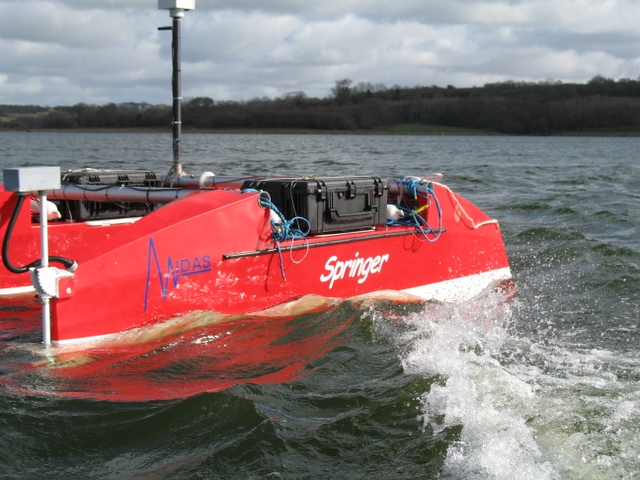
\includegraphics[width=\linewidth, height= 3.5cm]{./Images/USV/springer}
            \caption{The Springer}\label{fig:springer}
            \end{subfigure}
            \begin{subfigure}[b]{.40\linewidth}
            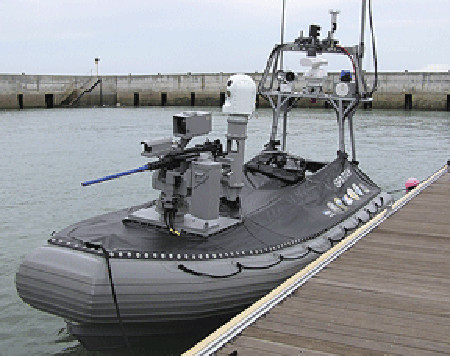
\includegraphics[width=\linewidth, height= 3.5cm]{./Images/USV/spartan}
            \caption{The Spartan}\label{fig:spartan}
            \end{subfigure}

            \begin{subfigure}[b]{.40\linewidth}
            \includegraphics[width=\linewidth, height= 3.5cm]{./Images/USV/barracuda}
            \caption{The Barracuda}\label{fig:barracuda}
            \end{subfigure}
            \begin{subfigure}[b]{.40\linewidth}
            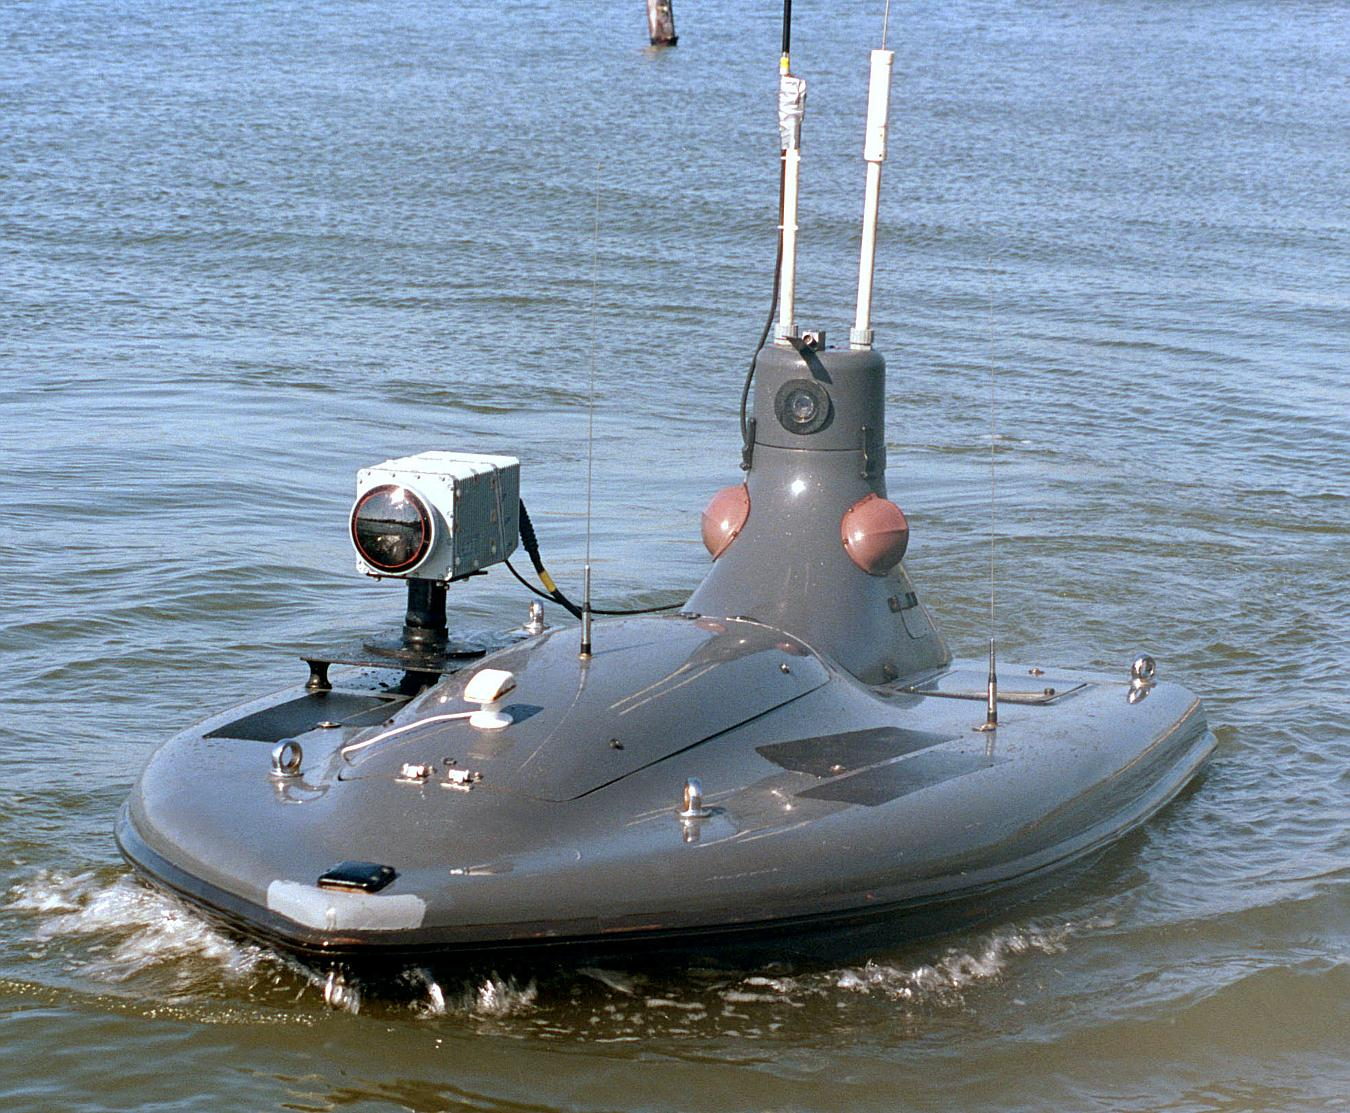
\includegraphics[width=\linewidth, height= 3.5cm]{./Images/USV/owl_mk2}
            \caption{The Owl}\label{fig:owl}
            \end{subfigure}
            \caption{Example of different USVs. In Fig.\ref{fig:springer} is represented the Springer, developed by Plymouth University for marine observation purposes. On the right, in Fig.\ref{fig:spartan} the Spartan, a multi\-mission reconfigurable USV built by SSC-San Diego. On the second row, on the left the canadian Barracuda (Fig.\ref{fig:barracuda}) while on the right, in Fig.\ref{fig:owl} the Owl MKII used for port security.}
      \end{figure}


      \indent Most of the vessel cited before are dual-purpose vehicles, meaning that they can be driven by humans, on-board or remotely, but also in an unmanned way. In this way their capabilities are augmented and extended in an affordable and low-risk manner.

      \indent To navigate in a fully autonomous way the presence of an \textit{obstacle avoidance module} is required to move the unmanned vessel from the actual track to another one if an immediate collision is expected, and then take it back on the previous one towards the goal pose (position and orientation). As it usually happens with ground robots, a path planner should be implemented: often it is distinguinshed in a \textit{global path planner} (GPP) and \textit{local path planner} (LPP). The goal of GPP is to find a safe path connecting the starting position, the actual pose of the robot, and the final one, called \textit{goal pose}. Sometimes in the literature it is also called a \textit{deliberative path planner}. Otherwise, the LPP has to react to immediate collision against unexpected obstacles, maybe not considered by the GPP, moving the autonomous vehicles far from the preplanned path in order to avoid the moving obstacle; for this reason it is also called \textit{reactive path planner}.

      \indent The structure of the paper is divided as follows: in Section \ref{obs_det} it will be illustrated how to perceive the environment surronding the autonomous vessel and detect static and moving obstacles with the most used computer vision techniques; in Section \ref{path_planner} it will be discussed more in details the necessity of having a robust path planner, therefore in Subsections \ref{gpp} and \ref{lpp} it will be illustrated how a global and a local path planners, respectively, could be implemented. Finally, in Section \ref{conclusion} a new combined path planner based on A* and Obstacle Velocity will be presented.


\section{Obstacle Detection} \label{obs_det}

      \indent To perfectly avoid obstacles moving across the path of autonomous vessels, an highly accurated world model is required. In order to obtain it, different sensors can be combined and data coming from them are usually fused in a 2D or 3D representation.

      \indent In \parencite{Almeida2009} the authors suggest to use an ARP radar sensor to identify moving obstacles and shores, and classify targets in terms of collision threat. They identify a set of perimeters, shown in Fig.\ref{fig:perimeters}, around the USV in order to decide appropriate measures: \textit{irrilevant} perimeter(3km), \textit{safe} perimeter(500m), \textit{warning} perimeter(250m) and \textit{prohibition} one(50m). Based on the \textit{closest point of approach} (CPA), defined as the estimated minimum distance between the detected object and the USV along its path, they classify targets as \textit{no threat} (CPA outside irrilevant perimeter), \textit{low threat} (CPA crosses the irrilevenat perimeter but not the safe one), \textit{potential threat} (CPA crosses the safe perimeter but not the prohibited one) and \textit{dangerous} (CPA inside the prohibition perimeter).

      \begin{figure}
            \centering
            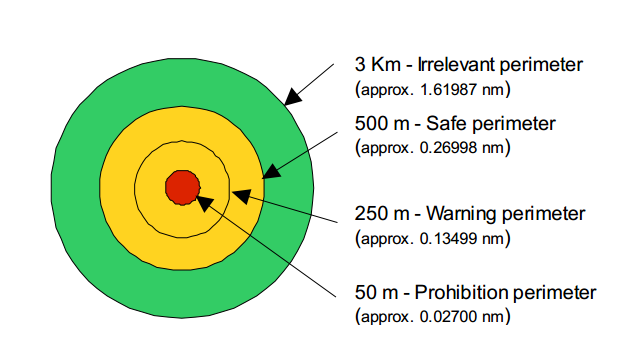
\includegraphics[height=5cm]{./Images/Almeida/perimeters}
            \caption{Multiple safety perimeters are drawn in the proximity of the USV. If the CPA of an obstacle is outside the irrelevant one, the obstacle is considered as \textit{no threat}; if the CPA is between the irrelevant and the safe perimeter, the obstacle is considered \textit{low threat}; if the CPA is between the safe and the warning perimeter, the obstacle is considered a \textit{potential threat}, while is considered \textit{dangerous} if it is inside the prohibition perimeter.}
            \label{fig:perimeters}
      \end{figure}

      \indent Low-cost radars are also used in the work of \textcite{Schuster2014}, in which an on-board collision avoidance module is required to compensate the lack of an automatic identification system (AIS).\\
      \indent In order to detect objects, data coming from radars need to be image preprocessing in the following way:
            \begin{itemize}
                  \item Ego Motion Compensation: the vessel's yaw rate is compensated calculating the azimuth of each scan in respect to the vessel's heading;
                  \item Occupancy Likelihood Determination: assuming that the probability \textit{p} of a cell being reported as occupied is independent and constant, the occupancy likelihood is binomially distributed;
                  \item Connected Component Labeling: adjacent occupied cells (whose occupacy probability is greater than 0.5) are grouped using connected component labeling \parencite{Gonzalez:2001:DIP:559707} to create an elliptical target.
            \end{itemize}
      Because the extracted target positions are very noisy, a low pass filter is adopted to get the object's true position, heading and velocity. To this scope, an \textit{Interactive Multiple Model} (IMM) filter is chosen: it runs several models in parallel and, based on the estimate of each model and the current measurement, a likelihood for each model to reflect the true motion state is determined. The output of the filter is a weighted sum of all model estimates and it is used by the collisions avoidance algorithm to predict the movement of the other vessels.\\
      The experiments conducted by the authors demonstrated a fast and robust technique for tracking obstacles on the sea surface, even if the accuracy in the position and velocity can be improved.

      \indent Other approaches use monocular and stereo vision methods for recording the presence of obstacles in proximity (30 to 100 m.) of the vessel. An example is offered by the work of \textcite{Wang2011,Wang2012}, that uses two cameras mounted parallel on a metal bar: the image from the camera on the left is initially used to perform monocular obstacle detection, and then the stero approach is applied to process the image from both cameras to compute the 3D detection results.\\
      The monocular technique is composed as follows:
            \begin{itemize}
                  \item Horizon Detection Module: it allows to distinguish the sea surface; it is realized using pixel profile analysis and Random sample consensus (RANSAC) \parencite{Fischler1981} method to perform line fitting (Fig. \ref{fig:line-fitting}) and extract the horizon (Fig. \ref{fig:horizon});
                  \item Saliency Detection Module: as expressed in \parencite{Achanta2009}, a binary mask is built and the detected salients will be given in the form of bounding boxes and considered of potential interest (Fig. \ref{fig:saliency});
                  \item Harris Corner Extraction and Tracking Module: using the work proposed in \parencite{Harris1988} and \parencite{Bouguet1999}, surface obstacles are distinguished among the potential identified previously (Fig. \ref{fig:corner});
                  \item Obstacle Detection Module: the data coming from the previous steps are combined to generate the final results (Fig.\ref{fig:monocular}); since it is pratical to measure the dynamics of a potential object to verify its validity as an obstacle, a tracked feature with long lifespan in the salient bounding box is labelled as of high priority and this link the obstacles in consecutive frames.
            \end{itemize}
      \indent The stereo correspondence phase could be divided in three: an initial phase in which both cameras are calibrated so the results are used for stereo image undistortion and 3D reconstruction, an intermediate phase in which \textit{epipolar constraint} reduces the 2D search for obstacle correspondence, and then a \textit{stereo matching} phase in which the normalized cross correlation template matching method is adopted. Here, the bounding box of obstacles by monocular obstacle detection in the left image is considered as the template window while the search is conducted along its epipolar line in the right image. In the end, a Kalman filter is applied on the horizontal disparity in order to eliminate the stereo matching error and improve the range estimation accuracy.\\
      This approach has shown good results until 100 m. far from the USV, despite low-resolution (640 x 480) images were used during the experiments. Therefore it is rational to believe that with more advanced cameras is it possible to improve the performance also for longer distance, even if increasing the image resolution means increasing the computation cost too.

      \begin{figure}
            \centering
            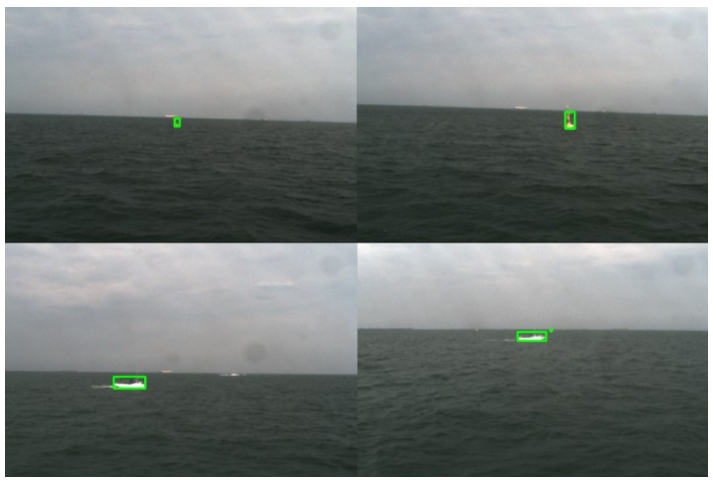
\includegraphics[height=5cm]{./Images/Wang/monocular}
            \caption{Results of the monocular obstacle detection approach in two different scenarios: in both cases, the obstacle is tracked among successive frames.}
            \label{fig:monocular}
      \end{figure}

      \begin{figure}
            \centering

            \begin{subfigure}[b]{.40\linewidth}
            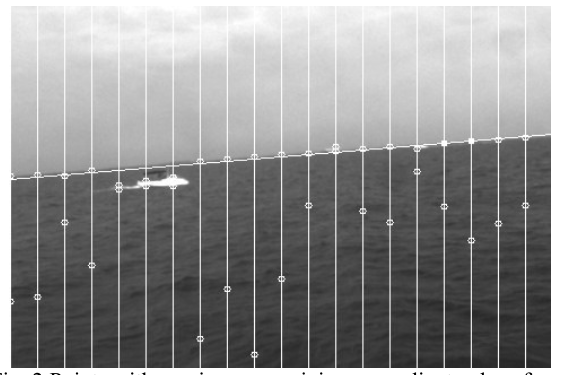
\includegraphics[width=\linewidth, height= 3.5cm]{./Images/Wang/line-fitting}
            \caption{}\label{fig:line-fitting}
            \end{subfigure}
            \begin{subfigure}[b]{.40\linewidth}
            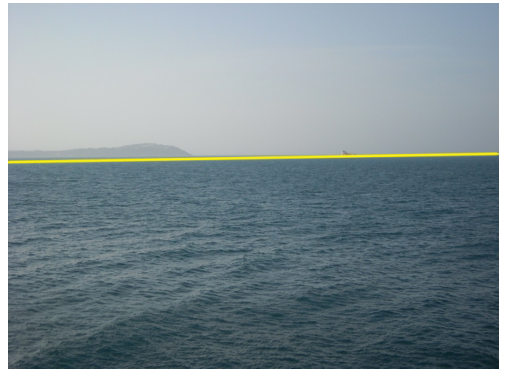
\includegraphics[width=\linewidth, height= 3.5cm]{./Images/Wang/horizon}
            \caption{}\label{fig:horizon}
            \end{subfigure}

            \begin{subfigure}[b]{.40\linewidth}
            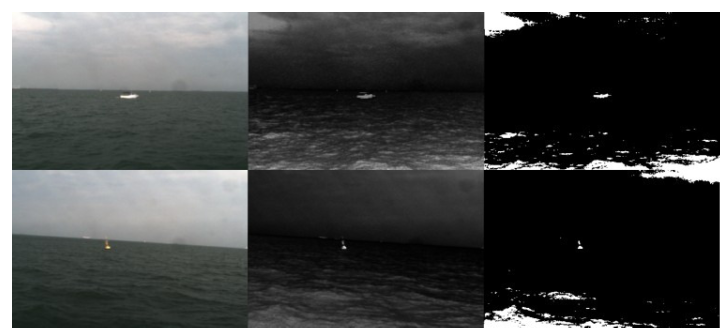
\includegraphics[width=\linewidth, height= 3.5cm]{./Images/Wang/saliency}
            \caption{}\label{fig:saliency}
            \end{subfigure}
            \begin{subfigure}[b]{.40\linewidth}
            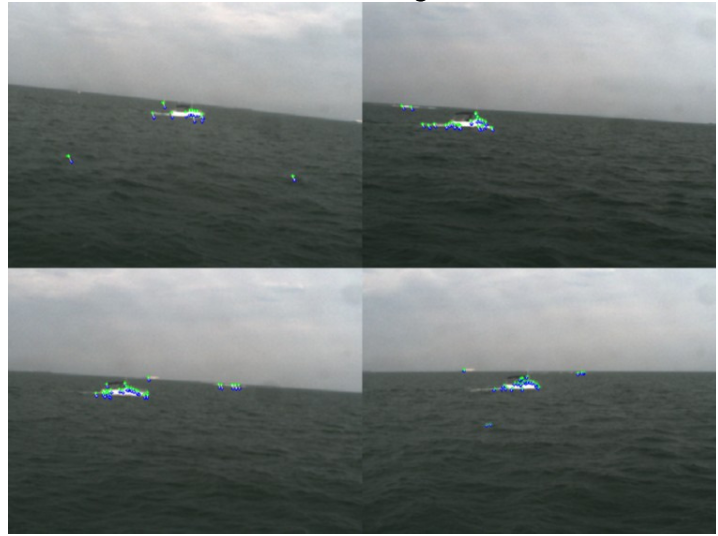
\includegraphics[width=\linewidth, height= 3.5cm]{./Images/Wang/corner}
            \caption{}\label{fig:corner}
            \end{subfigure}
            \caption{Monocular vision algorithm developed by \textcite{Wang2011}: in Fig.\ref{fig:line-fitting} the line separating sea and sky is fitted with the RANSAC method and then, in Fig.\ref{fig:horizon}, the horizon is extracted. Obstacles on the sea surface are identified with saliency detection, Fig.\ref{fig:saliency}, and their corner are extracted and tracked, as shown in Fig.\ref{fig:corner}}
      \end{figure}

      \indent A work similar to the previous one but that use only monular vision is the one proposed by Azzaby \textit{et al.} \parencite{Azzabi}. As before, the authors detect the horizon first and then the obstacles in the scene; last, they estimate the distance between the USV and objects, knowing the relative angle of each object and the horizion line. The algorithm developed for horizon detection can be summarized as follows:
            \begin{itemize}
                  \item Grey Level Transformation: the acquired image is transformed in grey scale to reduce image time processing (despite of a little loss of information) (Fig.\ref{fig:greyscale});
                  \item Sobel Operator: applied to the preprocessed image to identify those regions with high spatial frequency, mostly corresponding to edges \parencite{Maini2009} (Fig.\ref{fig:sobel});
                  \item Hough Transform: a line passing through two pixels in the image domain must lie on the intersection of two lines in Hough domain; in this way the edge detections is performed \parencite{Hough_1962};
                  \item Line Election: it chooses the couple (\textit{a,b}) for which the line passes through the maximum of points and then traces this line that will be probably the horizon line.
            \end{itemize}
      \indent After this, the next step is to detect objects in motion using \textit{optical flow estimation}: given an input stream, the velocity of each pixel is firstly calculated; if a pixel has a velocity higher than a threshold value and is under the horizon, it is marked as moving and tracked and in the end the optical flow vector of each pixel is plotted in the frame.\\
      \indent The output of the previous module is therefore used to estimate the distance from a USV to obstacles using a geometrical interpretation of the image.\\
      The contribution of this work is given by the use of greyscale image, and techniques that could be applied on it, to reduce the computational effort required by other algorithm such as \parencite{Ettinger2003} adopted in the work of \textcite{Larson2007a}.

      \begin{figure}
            \centering

            \begin{subfigure}[b]{.30\linewidth}
            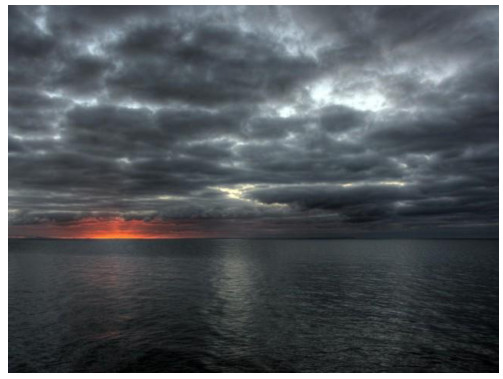
\includegraphics[width=\linewidth, height= 3.5cm]{./Images/Azzabi/original}
            \caption{Original image}\label{fig:original}
            \end{subfigure}
            \begin{subfigure}[b]{.30\linewidth}
            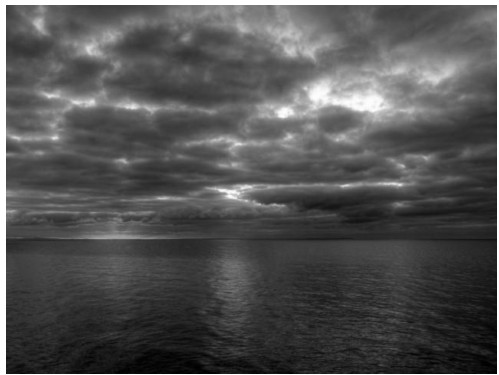
\includegraphics[width=\linewidth, height= 3.5cm]{./Images/Azzabi/greyscale}
            \caption{Greyscale image}\label{fig:greyscale}
            \end{subfigure}
            \begin{subfigure}[b]{.30\linewidth}
            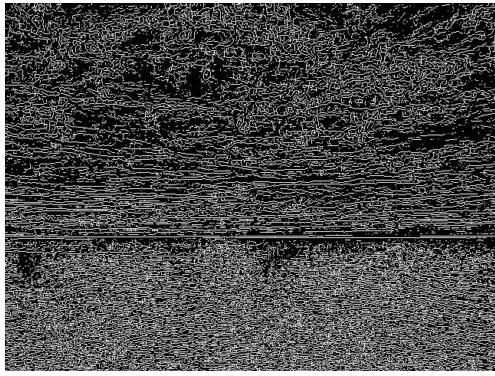
\includegraphics[width=\linewidth, height= 3.5cm]{./Images/Azzabi/sobel}
            \caption{Sobel transformation}\label{fig:sobel}
            \end{subfigure}

            \caption{In \parencite{Azzabi} the obstacles edges are identied firstly grey-transforming the monocular image (Fig.\ref{fig:greyscale}) and then applying the Sobel operator (Fig.\ref{fig:sobel})}
      \end{figure}

\section{Path Planner} \label{path_planner}

      After having perceived the surrounding environment and the obstacles present in it with the techiques previously described,a model of the world should be realised. This can be done in a two or three dimensional space but often the first option is preferred because it can guarantee less computational time to operate with it. Having a virtual representation of the world is a key point to plan a path for moving the autonomous vessel.\\
      As described in Section \ref{introduction},  the Path Planner module is usually divided in two sub-components: the global path planner aims to find a path from the actual pose of the robot to a goal one, while the local path planner tries to avoid moving obstacles close to the robot.\\
      \indent In the following subsections it will be described the most recent path planners used in marine robotics, to guide autonomous vessels on the sea surface among other marine crafts and moving hazards.

        \subsection{Global Path Planner} \label{gpp}

              The goal of the GPP is to continuosly modify the existing waypoint route to plan around obstacles detected with the long-range sensors. In the work of \textcite{Larson2007,Larson2007a}, the path planners use a two-dimensional (2D) obstacle map created by dividing the environment into a discrete grid and assigning each cell location a value representing the probability of being occupied or not by an obstacle. This is filled with stationary obstacles from the \textit{chart server} and moving obstacles provided by the radar. The underlying search technique is the A* search algorithm \parencite{4082128}, chosen because it can find an optimal solution in a short amount of time. Since A* uses a cost analysis at each step, Larson \textit{et al.} inserted an added cost for proximity to obstacles for allowing a USV to set a safety barrier around obstacles.\\
              To avoid moving obstacles, the path planner determines safe velocity ranges using the \textit{Velocity Obstacles} (VO) method (Fig.\ref{fig:obs_vel}): a velocity space \textit{v-$\theta$} grid (where \textit{v} denotes the USV speed and \textit{$\theta$} is the heading angle) is constructed as decision space to find the best velocity vector and the moving obstacle is expanded by the robot size. The reason to do this it to treat the robot as a point. As long as the robot's velocity lies outside the VO, it will not collide with obstacle, assuming that the velocity vectors are constant over time; if the velocity obstacle change over time, the VO-based approach reacts by replanning using the latest sesnsor information.\\
              In the case that changing the velocity does not avoid collision, the path planner changes path by creating a \textit{projected obstacle area} (POA) (Fig.\ref{fig:poa}), for each obstacles and determining a safe alternative route using a A* search. A POA is the area a moving obstacle could occupy in the future. This area is identified calculating the CPA: since a moving obstacle can pose a threat to the USV along multiple stretches of the path, it is necessary to calculate the CPA of every obstacle along each path segment.

              \begin{figure}
                    \centering
                    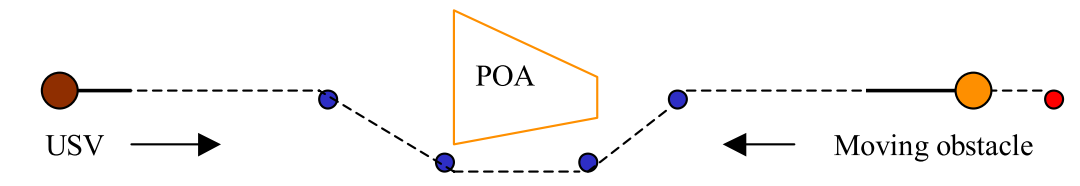
\includegraphics[width=\columnwidth]{./Images/Larson/poa}
                    \caption{The USV has to avoid the obstacle coming ahead passing port-to-port its projected obstacle area.}
                    \label{fig:poa}
              \end{figure}

              \begin{figure}
                    \centering
                    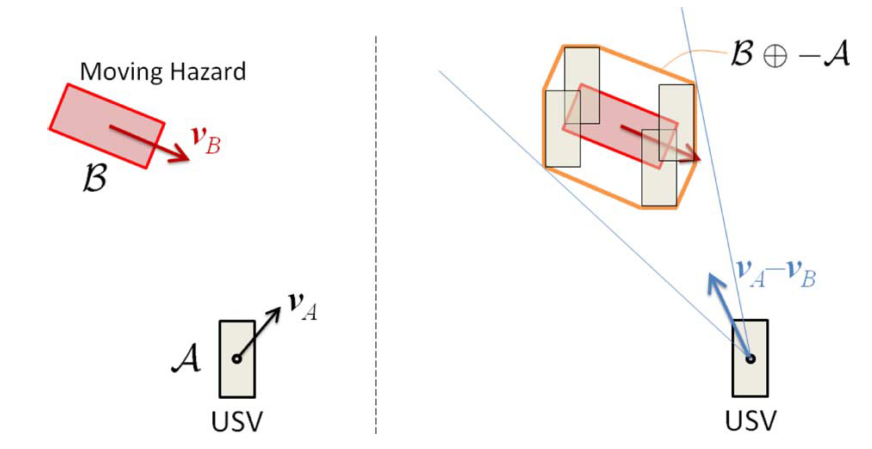
\includegraphics[height=5cm]{./Images/Kuwata/obs_vel}
                    \caption{To avoid the collision, the relative velocity $\vec{v_A}$ - $\vec{v}_B$ has not to be inside the cone formed by the robot center and the expanded obstacle $A\oplus B$.}
                    \label{fig:obs_vel}
              \end{figure}

              Among the previous concepts, the authors decided also to consider the International regulations for preventing collisions at sea (known as COLREGS, for COLlision REGulationS). In this work the authors consider three primary COLREGs, shown in Fig.\ref{fig:colregs}: crossing, overtaking and head-on situations. In the situation in which a traffic boat is crossing from the right, the vessel with the other on its starboard (right) side must give away. In the case of a USV overtaking a slow traffic boat, it must ensure enough clearance so that it keeps out of the way of the traffic boat being overtaken. Otherwise, if the USV and the traffic boat are moving straight toward each other, both vessels must alter their course toward the starboard, so that they pass with the other vessel to its port(left side).\\
              The POA of a moving obstacle is calculated from the current path of the USV and the time taken to traverse that path. As the path changes, there is a need to update the POA and recalculate.

              \begin{figure}
                    \centering
                    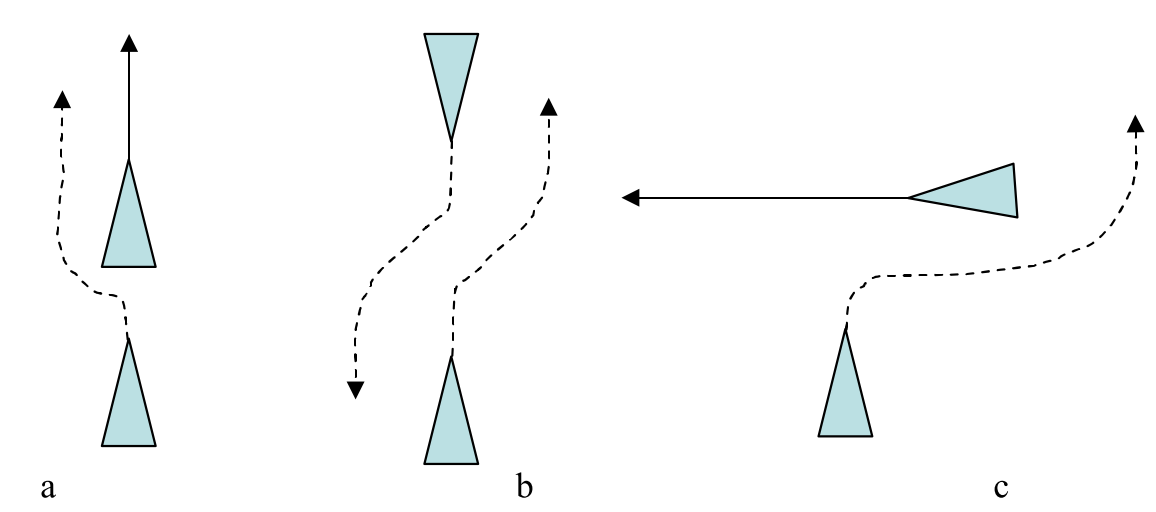
\includegraphics[height=5cm]{./Images/Larson/colregs}
                    \caption{Rulsed defined to avoid collisions for overtaking (a), meeting (b), and crossing (c) obstacle.}
                    \label{fig:colregs}
              \end{figure}

              \indent \textcite{Casalino2009} suggest an approach based on the \textit{Visibility Graph} (Fig.\ref{fig:visibility}) concept and on a world-model in which obstacles are polygons and the robot is a point. A visibility graph is a graph of intervisible locations, typically for a set of points and obstacles in the Euclidean plane. Each node in the graph represents a point location, and each edge represents a visible connection between them. That is, if the line segment connecting two locations does not pass through any obstacle, an edge is drawn between them in the graph.\\
              In order to use the Visibility Graph the obstacles inside the working area had to be transformed into polygons. At this point the Dijkstra's Algorithm \parencite{EWD:NumerMath59} is applied between the starting point and the goal one and the resulting trajectory will not intersect any of the obstacles.


              \begin{figure}
                    \centering
                    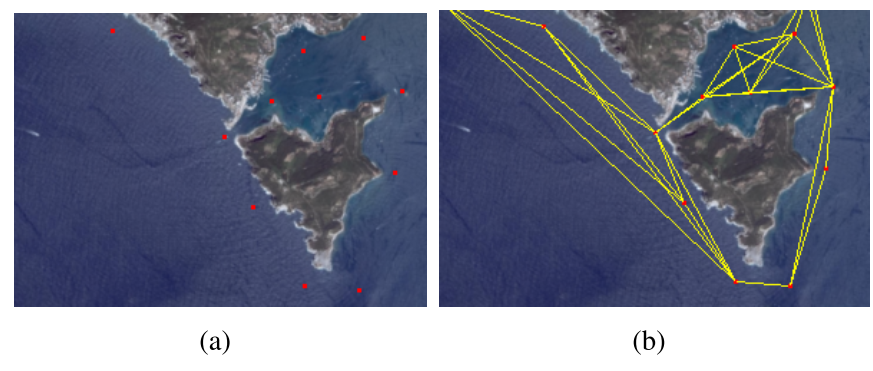
\includegraphics[height=5cm]{./Images/Casalino/visibility_graph}
                    \caption{A visibility graph is built identifying first a list of vertices (a) and then connect those nodes visible one from each other.}
                    \label{fig:visibility}
              \end{figure}

              A totally different approach has been developed by \textcite{Xie2014}. The authors take inspiration from the concept of \textit{Artificial Potential Field} (APF) \parencite{Khatib1985} and improved it to be more robust such that it can avoid local minima, destinations unreachable and poor accuracy. APF consists in combining the repulsion potential field of obstacles and gravitational potential field of targets in the operational space.\\
              In the APF model,shown in Fig.\ref{fig:apf}, $T$ represents the target which produces the attraction to the USV, $O$ represents obstacles which produce repulsion to the USV. If $X_d$ represents the target position, the control of the USV with respect to the obstacle $O$ can be carried out in the artificial potential:

                  \begin{equation} \label{eq:apf}
                         U_{art}(x) = U_{att}(x) + U_{rep}(x)
                  \end{equation}

              where $U_{art}$, $U_{att}$, $U_{rep}$ represent artificial potential field, attraction potential field and repulsion potential energy respectively.\\
              The improvement introduced consists in a regulatory factor that, in the presence of an obstacle, controls attraction for decreasing as a linear factor and repulsion as a higher-order function. In this way, the USV will not encounter the case of local minum or destination unreachable, but it demonstrated in simulation to be able to avoid obstacles smoothly and reach the goal.

              \begin{figure}
                    \centering
                    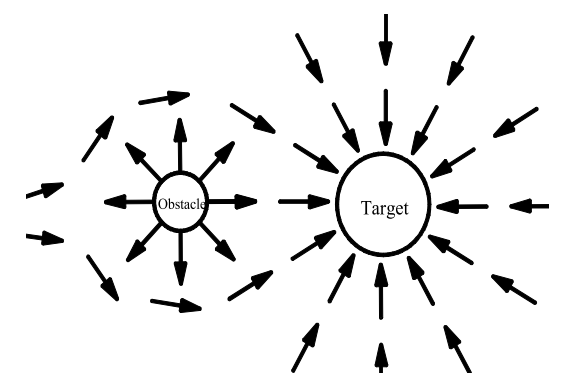
\includegraphics[height=5cm]{./Images/Xie/apf}
                    \caption{The model of APF}
                    \label{fig:apf}
              \end{figure}

              \textcite{Conference2013} adopt in their work a Micron DST sonar as the obstacle avoidance sensor. They propose a method in which the scanning angle can adapt to the distance from the sonar to the obstacle. The fuzzy logic algorithms are used to make the strategy timely and effective. Their approach is described as follows:
                    \begin{itemize}
                          \item Data Collection and Pretreatment: interesting byte are extracted from the sonar packages to reduce computational complexity;
                          \item Noise Reduction: noise caused by ambient affection is reduced by a threshold filter;
                          \item Obstacle Avoidance Algorithm Design: the scan range is set to four levels; if no obstacle is detected in a cycle, the scan range will jump to the upper level, otherwise the scan range will down to the nearest level which is bigger than the distance from obstacle to the sonar head. At this point, the type of the obstacle line is determined and the slope is calculated and sent to the next module;
                          \item Decision-making Module: in order to make the route timely and effective, fuzzy technology is used in motor control;
                    \end{itemize}
              This work shows good results and the model used during experiments always avoided obstacles and shores. The only limitation encountered by the authors was given by the low precision of inertial navigation system used which compromise the accuracy of the reaction.

        \subsection{Local Path Planner} \label{lpp}

              A first example of LPP is given by the work of Kuwata \textit{et al.} \parencite{Kuwata2014}, in which the authors suggest an algorithm to not only address hazard avoidance for stationary and moving hazards, but that also applies the COLREGS. In this work, as in \parencite{Larson2007}, the authors consider three primary COLREGS: crossing, overtaking and head-on situations.\\
              Moreover, the proposed approach use the Velocity Obstacle (VO) concept: in this way a moving obstacle is transformed  into a stationary one by considering the relative velocity and trajectory of the USV wih respect to the obstacle, and in the end it returns a set of USV velocity vectors guaranteeing collision avoidance.\\
              The developed algorithm works in this way:
                    \begin{itemize}
                          \item Precollision Check: the closest point of approach (CPA) is computed with the current position and velocity of the USV and traffic vessels, and it is evaluated if any COLREGS rules need to be applied;
                          \item Rule Selection: if the CPA meets temporal and distance conditions, the best COLREGS rule is applied analyzing a set of geometric constraints;
                          \item Hysteresis: introduced to lower the rate at which the USV can change what rules to apply; this means that once a COLREGS maneuver is initiated, it continues to direct the boat for at least a minimun duration of time;
                          \item Cost: once the constraints set of VO and COLREGS are generated, a defined cost for each \textit{$v_i$} and \textit{$\theta_j$} ammissible is generated and the (\textit{$v_i$}, \textit{$\theta_j$}) pair with the minimum cost is selected and the velocity command is sent to the vehicle controller.
                    \end{itemize}

              \indent A similar approach has been implemented by Leng \textit{et al.}. In \parencite{Leng2013} the Velocity Obstacle approach is integrated with Mixed Linear Integer Programming (MILP). In solving the path planning problem, the dynamics and kinematics of the USV, sensors and uncertainty constraints of the environment all can be taken into consideration and linearized. In the end, the objective function will be
                  \begin{center}
                    min: $ \mid $ \textit{L$_{UG}$} - (\textit{v$_{UG}$} + \textit{$\Delta$ v$_{UG}$})$\Delta$t $ \mid$
                  \end{center}
              where \textit{L$_{UG}$} and \textit{v$_{UG}$} denote the relative distance and velocity between the USV and the target point.\\
              As in \parencite{Kuwata2014}, the collision is checked calculating the the CPA and its distance from the vessel. After this, six types of encounter situations are identified and the USV reacts depending on this decision.

              \indent Also the authors of \parencite{Larson2007,Larson2007a} describe a local or \textit{reactive} path planner module; in their work, in addition to the global path planner described in Subsection \ref{gpp}, a local one is required because the long-range sensors are not capable of detecting small low-profile obstacles such as very small personal boats, or because the USV may inadvertently deviate from the planned path if GPS is jammed or the Inertial Navigation Unit (INU) drifts. \\
              In the adopted approach, all the near-field sensors are fused into a common level world-model, and individual behaviors vote on specific navigation solutions within that model. A number of arcs are projected in front of the vehicle over the local world-model obstacle map. The number of arcs considered is a function of the map size and grid spacing, with the arcs spaced such that one arc pases through each of the outer cells. \\
              This approach guarantees that each cell in the grid is covered by at least one arc so that all the navigable path are considered. Each arc is given a weight or vote based on the distance the robot could travel along the arc before it encountered an obstacle. The votes are scalded from 0 to -1 so that they can be combined with votes from oher navigation behaviors.

              \indent In \parencite{Casalino2009} a new reactive path planner based on the \textit{bounding box} concept is described. A bounding box of a track is easily defined as the rectangle that defines the area the USV should avoid in order to guarantee a safety distance from the moving object. The algorithm proposed suggests to integrate the USV actual position $S$ and the local goal $G$ to a graph made of the four edges of the box, by adding the edges starting from either $S$ or $G$ and ending on one of the vertexes of the box that are not intersecting any edge. Then the solution would be any path from $S$ to $G$, which can be obtained by any graph taversing algorithm, such as A* or Dijkstra's algorithm. The problem with this approach is its sub-optimality because it does not take into account any kinematic property of the tracks nor the USV.\\
              The algorithm implemented to reach the locally optimal avoidance is composed as follows, using an A* search:
                    \begin{itemize}
                          \item For each visible vertex of the bounding box, compute the angle $\theta$ such that the vessel can intercept it;
                          \item Calculate time(cost) \textit{$\bar{t}$} and position $\bar{P}$ of intercept;
                          \item Calculate estimated time to goal \textit{h} $\equiv$ \textit{G} - \textit{$\bar{P}$} / \textit{$v_1$}, where \textit{$v_1$} is vehicle's speed;
                          \item Compute global estimate cost \textit{f} = \textit{$\bar{t}$} + \textit{h}.
                    \end{itemize}
              At each iteration the node with the lowest \textit{f} is selected and popped from the \textit{openset}, the set of all the nodes that have been created but not yet explored in the search. It's therefore checked whether the goal can be reached without collision: if so end the search. Otherwise, for each obstacle, calculate the vertexes intercept positions and check if this path is collision free with \textit{ray tracing} techinque. If so, add this node to the openset and proceed back to the first step.

              \indent In the successive work \parencite{Simetti2014} the authors present a refinement of this algorithm. To avoid crossing the bounding box and thus failing the obstacle avoidance, they introduce a \textit{safety bounding box} around the original collision bounding box. All the computations are now performed against it, and its vertexes are used to performed the avoidance. If for same reasons the USV enters the safety box, it must exit it without crossing the main diagonals, ensuring that the vehicle moves away from the collision bounding box.\\
              To increase the likelihood that the path is still collision free with the safety bounding box even under estimation uncertainty, a \textit{supporting bounding box} is adopted, whose dimensiond depends on the position of the USV:
                    \begin{itemize}
                          \item if the USV is inside the safety bounding box, the supporting one coincides with the safety one;
                          \item if the USV is far away with the safety bounding box, the supporting one coincided with a maximum bounding box;
                          \item if the USV is in-between the maximum bounding box and the safety one, the supporting one varies with the distance, shrinking as the USV is closer to the safety one.
                    \end{itemize}
              In this way, when the USV if far away from the incoming vessel, the computed path will be very robust to changes in speed and heading of the obstacle and its safety bounding box.

              A different approach based on lane-constrained trajectory generation is proposed in \parencite{Tan2010}. Here, while avoiding obstacles, the vessel has to meet some objectives. Firstly, it is required to maintain a minimum distance from each obstacles at all times (\textit{safety distance} objective). Secondly, the USV must observe the COLREGs rules. The last two objectives are called \textit{cross track} and \textit{shortest time} objectives: they means the USV should keep as close as possible to the intended path and complete it the the shortest path possible.\\
              The idea presented is divided in two step:
                    \begin{itemize}
                          \item Maneuver Generation: the platform's motion is forward simulated for a fixed number of time steps using simple models of the maneuvers tracker and the boat;
                          \item Maneuver Selection: is a multi-stage process in which objectives, divided in \textit{rules} and \textit{criteria}, are ordered based on fixed priorities. At each stage, a single objective is considered and candidate are eliminated based on that particular objective; as long as more than one candidate emrges from the elimination, the remaining candidates are subjected to the next stage of elimination.
                    \end{itemize}
              A limitation of this approach is given by the generation step: because only a sample of possible maneuvers is taken, the algorithm may sometimes be unable to find a solution.

              \indent In \parencite{Blaich2015} it's proposed a specialized A* algorithm that allows velocity variations and considers different turning circles for different velocities. First of all, a three-dimensional occupancy grid is built by inserting the measurementd of the laser finder which are transformed to a local reference frame. Then the map is processed and contours of obstacles are extracted.\\
              In parallel to the mapping procedure for static obstacles, a \textit{Multi Object Tracket} (MOT) is implemented for moving objects.\\
              For the evasive path generation, an A* algorithm is specialised such that it considers static obstacles, tracked agents and the mission path. A penalty depending on the total lenght of the path that had to be skipped is added to the cost function of the A* algorithm. This results in evasive path that lead back to the mission path after avoiding an obstacle. However, to guarantee the feasibility of an evasive path, the kinematic constraints of the USV have to be considered during the path search. To use the full dynamic capability of the vessel, it is necessary to allow changing velocities in the evasive path along with the respective changes of the minimum turning circle. These alternations in velocity are enabled by adding both the velocity and the time to the search space, that consist now of four dimensions - two for position and one dimension for each time and velocity.

              Tang \textit{et al.} in \parencite{Tang2012} shows a new method called \textit{Obstalce Avoidance Algorithm Based on Heading Window} (OAABHW) for the near-field static obstacle avoidance of USVs. The algorithm transforms dynamic windows into heading window and translational velocity window by using \"Divide and Conquer\" Strategy, and grasp an optimized avoidance angle from solving the constraint optimization problem of heading window at second step. Then the rotational velocity could be determined by the navigation angle and heading of USV. The translational velocity of avoidance is produced by the translational velocity model which is formed by the rotational velocity and the distribution of obstacles in the surroundings.\\
              Based on the concept that the translational velocity is less important than the heading angle, the authors build the relative coordinate of USV and upload all the obstacles to it. Then the constraint set of heading angle of USV can be calculated by dealing the obstacle in near-field on tangent method. Obstacles are replaced by their circumcircle, and the geometry size of the USV is regarded as the expanded factor of obstacle expanding, meanwhile USV can be treated as a particle.\\
              In the near-field of USV, a number of virtual rays projected around the USV with a certain angular resolution, any angle obstructed by obstacles is defined as infeasible heading angle of USV. Upon the analysi of obstalces in the relative coordinate of USV by tangent method, the maximum angle and minum angle could be grasped and recored as $\theta_{obs\_max}$ and $\theta_{obs\_min}$. Then these two angles are transferred from relative coordinate to absolute ones.\\
              In the process of excellent heading angle selection, the degree of heading yaw is treated as optimization objective. The heading window and the infeasible set of heading angle are treated as constraints. By solving the single optimization problem, the best navigation angle can be grasped. The constrain set optimzation problem can be mathematically formulated as:
                  \begin{center}
                        $max: F_{Head} (\theta) = 1 - \frac{\theta_{goal} - \theta}{2\pi}$
                  \end{center}
              where $\theta_{goal}$ is the basic value of optimal angle selection which is formed by global target point and the current position of USV.\\
              The excellent avoidance navigation angle $\theta_{out}$ is obtained and the avoidance rotational velocity $\omega_{out}$ could be calculated by it and the current heading angle $\theta_{USV}$:
                  \begin{center}
                        $\omega_{out} = \omega_c + \frac{2(\theta_{out} - \theta_{USV} -\omega_c * \Delta t)}{\Delta t}$
                  \end{center}
              where $\omega_c$ is the current rotational velocity of USV, and $\Delta t$ is time\-window.\\
              The translational velocity strongly depends on the rotational one and on the obstacles distributions. If obstacles are close to USV or the avoidance rotational velocity $\omega_{out}$ is comparatively large, then it has to slow the translational velocity to pass the hazard areas. If obstacles are far away from USV and rotational velocity is small, then USV should navigate at high speed.

              \indent Because in real marine environments the trajectory of the vessels is influenced by many factors such as sea wind, currents and waves, Zhang \textit{et al.} in \parencite{Zhang2014} illustrate a new adaprive obstalce avoidance algorithm based on Sarsa on-policy reinforcement learning (AABSRL).\\
              It is composed of two modules: the local obstacle avoidance module (LOAM) focuses on obstacle avoidance in the environmente and ignores external disturbance factors, while the disturbances from sea wind and currents are dealt with in the adaptive learning module (ALM). The responsability of ALM is to search for a course compensation angle to offset the course deviation angle that is generated by external disturbance factors. Its core is composed by the Sarsa on-policy reinforcement learning-based adaptive learning algorithm, which is used to explore the course compensation angle of USV. The input data of ALM include the state data of USV, the state data of sea wind and currents, and the guidance angle from LOAM. This one is realised using the OAABHW algorithm presented in \parencite{Tang2012} and previously described in this paper.\\
              Under the disturbances of sea wind and currents, the course angle deviates from the guidance angle. To keep the safe navigation of USV, the ALM of AABSRL needs to search for a certain course compensation angle $\Delta \theta_H $ to offset the course deviation. The Boltzamann distribution-based selection strategy is used to select the action of course compensation angle in the learning process, because it is typically greedy in the limit and infinite exploration (GLIE). Moreover, under thiese assumptions it can converge to the optimal action strategy with probability 1.



\section{Conclusion} \label{conclusion}



%----------- IEEE JOURNAL BEGIN -----------
\begin{comment}
\ifCLASSOPTIONcaptionsoff
  \newpage
\fi
\end{comment}
%----------- IEEE JOURNAL END -------------
% references section

%\bibliography{bibliography}
%\bibliographystyle{plain}
\printbibliography



% that's all folks
\end{document}
